%NOTE! compile with XeLaTeX
\documentclass[a4paper, 12pt]{report}

\usepackage[left=3.0cm, right=1.5cm, top=2.0cm, bottom=2.5cm]{geometry}
\usepackage[utf8]{inputenc}
\usepackage{ragged2e}

\usepackage{titlesec}
\usepackage{tocloft}

\usepackage{setspace}
\usepackage[numbers]{natbib}
\usepackage{fancyhdr}
\usepackage[hidelinks]{hyperref}
\usepackage[none]{hyphenat} %որ տողադարձ չանի

\usepackage{amssymb} % for additional math environments and symbols
\usepackage{amsmath}

%Հայերենի համար անհրաժեշտ բաղադրամասեր
\usepackage{fontspec}
\usepackage{polyglossia}
\setdefaultlanguage[numerals=arabic]{armenian}
\newfontfamily\armenianfont{GHEA Mariam}

% Adjust font size and centering for \bibname
\titleformat{\chapter}[display]
{\bfseries\centering}{\chaptertitlename\ \thesection}{1em}{}

\linespread{1.5} % միջտողային հեռավորությունը
\setlength{\parindent}{0cm} % Նոր պարբերությունը 0սմ հեռավորությունից սկսել

% Բովանդակության համարակալման և տեսքի համար
\renewcommand{\thesection}{\arabic{section}.}
\renewcommand{\thesubsection}{\thesection\arabic{subsection}.}
\renewcommand{\thesubsubsection}{\thesubsection\arabic{subsubsection}.}

% Վերնագրերը տեքստում գրվեն մեջտեղից և մուգ
\titleformat{\section}
{\bfseries\centering}
{\thesection}
{1em}
{}

\titleformat{\subsection}
{\bfseries\centering}
{\thesubsection}
{1em}
{}

\titleformat{\subsubsection}
{\bfseries\centering}
{\thesubsubsection}
{1em}
{}

% Adjust spacing for section headers
\titlespacing*{\section}{0pt}{1cm}{1cm}
\titlespacing*{\subsection}{0pt}{1cm}{1cm}

% Bold fonts for table of contents
\renewcommand{\cftsecfont}{\bfseries}
\renewcommand{\cftsubsecfont}{\bfseries}

\renewcommand{\contentsname}{Բովանդակություն} %որ contents-ի փոխարեն հայերեն գրի
\renewcommand{\cfttoctitlefont}{\bfseries} % որ Բովանդակությունը գրվի փոքր և մուգ տառերով

\renewcommand{\bibname}{Գրականություն} %որ references-ի փոխարեն հայերեն գրի

\sloppy %ձախից և աջից հավասարեցում
\usepackage{indentfirst}
\setlength{\parindent}{1cm} % Գրել մի մատ խորքից

\begin{document}
    \pagenumbering{gobble} % Անջատել էջերի համարակալումը
    \begin{titlepage}
    \begin{center}
        \linespread{1.3}
        \vspace{0.5cm}
        {
            \fontsize{18}{0}
            \textbf{ԵՐԵՎԱՆԻ ՊԵՏԱԿԱՆ ՀԱՄԱԼՍԱՐԱՆ} \\
        }
        \vspace{1cm}
        {
            \fontsize{18}{0}
            \textbf{ՏԵՂԵԿԱՏՎԱԿԱՆ ՏԵԽՆՈԼՈԳԻԱՆԵՐԻ ԿՐԹԱԿԱՆ ԵՎ ՀԵՏԱԶՈՏԱԿԱՆ ԿԵՆՏՐՈՆ} \\
        }
        \vspace{1cm}
        {
            \fontsize{16}{0}
            \textbf{ՏԵՂԵԿԱՏՎԱԿԱՆ ՀԱՄԱԿԱՐԳԵՐԻ ԱՄԲԻՈՆ} \\
        }
        \vspace{1cm}
        {
            \fontsize{18}{0}
            \textbf{ՏԵՂԵԿԱՏՎԱԿԱՆ ՀԱՄԱԿԱՐԳԵՐԻ ԿԱՌԱՎԱՐՈՒՄ ԿՐԹԱԿԱՆ ԾՐԱԳԻՐ} \\
        }
        \vspace{2cm}
        {
            \fontsize{18}{0}
            \textbf{Մկրտչյան Ալբերտ Կարենի} \\
        }
        \vspace{1.5cm}
        {
            \fontsize{18}{0}
            \textbf{ՄԱԳԻՍՏՐՈՍԱԿԱՆ ԹԵԶ} \\
        }
        \vspace{1cm}
        {
            \fontsize{16}{0}
            \textbf{Ծրագրային կոդի հատկությունների հարցումների համակարգ} \\
        }
        \vfill
        {
            \fontsize{14}{0}
            \textbf{\textit{«Տեղեկատվական համակարգերի կառավարում» մասնագիտությամբ ինֆորմատիկայի մագիստրոսի որակավորման աստիճանի հայցման համար}} \\
        }
        \vspace{1cm}
        {
            \fontsize{13}{0}
            \textbf{ԵՐԵՎԱՆ 2024} \\
        }
    \end{center}
\end{titlepage}

        {
        \linespread{1}
        {
            \large
            \raggedright
            \parbox[t]{2.5cm}{\fontsize{13}{0}\textbf{\textit{Ուսանող՝}}}
            \parbox[t]{0cm}{\underline{\hspace{4cm}} \scriptsize\makebox[4.1cm][c]{\textit{Ստորագրություն}}} \hfill
            \parbox[t]{9.5cm}{\fontsize{13}{0}\textbf{\textit{Մկրտչյան Ալբերտ}}} \\
        }

        \vspace{2cm}
        {
            \large
            \raggedright
            \parbox[t]{5.2cm}{\fontsize{13}{0}\textbf{\textit{Գիտական ղեկավար՝}}}
            \parbox[t]{0cm}{\underline{\hspace{4cm}} \scriptsize\makebox[4cm][c]{\textit{Ստորագրություն}}} \hfill
            \parbox[t]{6.9cm}{\raggedright\fontsize{13}{0}\textbf{\textit{ֆ.մ.գ.թ., Ասլանյան Հայկ}}} \\
        }

        \vspace{2cm}
        {
            \large
            \raggedright
            \parbox[t]{2.5cm}{\fontsize{13}{0}\textbf{\textit{Գրախոս՝}}}
            \parbox[t]{0cm}{\underline{\hspace{4cm}} \scriptsize\makebox[4cm][c]{\textit{Ստորագրություն}}} \hfill
            \parbox[t]{9.5cm}{\fontsize{13}{0}\textbf{\textit{ֆ.մ.գ.թ., դոցենտ, Մանուկյան Մանուկ}}} \\
        }


        \vfill
        {
            \large
            \raggedright
            \fontsize{13}{0}
            \textbf{\textit{«Թույլատրել պաշտպանության»}}
        } \\

        \vspace{2cm}
        {
            \large
            \raggedright
            \parbox[t]{3.9cm}{\fontsize{13}{0}\textbf{\textit{Ամբիոնի վարիչ՝}}}
            \parbox[t]{2cm}{\underline{\hspace{4cm}} \scriptsize\makebox[4cm][c]{\textit{Ստորագրություն}}} \hfill
            \parbox[t]{8cm}{\raggedright\fontsize{13}{0}\textbf{\textit{ՀՀ ԳԱԱ ակադեմիկոս, ֆ.մ.գ.դ., պրոֆեսոր, Սամվել Շուքուրյան}}} \\
        }

        \vspace{1.5cm}
        {
            \raggedright
            \large
            \textit{«}\underline{\hspace{1.5cm}}\textit{»}\underline{\hspace{2.5cm}}20\underline{\hspace{0.5cm}}\textit{թ} \\
        }

        \newpage
    }

    \clearpage
    {
	\thispagestyle{plain}
	\begin{center}
		\large
		\textbf{Համառոտագիր}
	\end{center}

	\begin{center}
		\vspace{0.5cm}

		\large
		\textbf{Ծրագրային կոդի հատկությունների հարցումների համակարգ հիմնված ղեկավարման կախվածությունների գրաֆի վրա}

		\vspace{0.2cm}
		\textbf{Система запроса свойств исходного кода на основе графа зависимостей управления}

		\vspace{0.2cm}
		\textbf{A system for querying source code properties based on a control dependency graph}

		\vspace{0.5cm}

	\end{center}
	Աշխատանքի շրջանակներում հետազոտվել են կախվածությունների գրաֆներ կառուցող ժամանակակից գործիքները։
	Գոյություն ունեցող գործիքները կախվածությունների գրաֆներ կառուցելու համար կատարում են ղեկավարման և
	տվյալների հոսքերի վերլուծություններ կոդի միջանկյալ ներկայացման հիման վրա։ Սակայն երբ ծրագրի նախնական
	կոդի մի մասը հասանելի չէ, մինջանկյալ ներկայացման թարգմանությունը հնարավոր չէ կատարել։ Աշխատանքում
	նախագծվել ու իրականացվել է գործիք, որը թույլ է տալիս շարահյուսորեն վերլուծվող նախնական կոդի համար
	կառուցել կախվածությունների գրաֆներ։
}

    \newpage
    \begin{center}
        \tableofcontents
    \end{center}

    \pagenumbering{arabic} % Միացնել էջերի համարակալումը
    \setcounter{page}{4} % համարակալումը սկսել 4-ից

    \clearpage
    \phantomsection
    \section*{\textbf{ՆԵՐԱԾՈՒԹՅՈՒՆ}}\label{sec:introduction}
    \addcontentsline{toc}{section}{ՆԵՐԱԾՈՒԹՅՈՒՆ}
    {
	Ստեղ կլինի ներածության տեքստը
}


    \section{Արդիականություն}\label{sec:modernity}
    {
    \section{Արդիականություն}\label{sec:modernity}
    Աշխարհում առկա ծրագրային կոդի հատկությունների վերլուծության գործիքներն ունեն որոշ սահմանափակումներ և թերություններ:
    Այդ գործիքների մեծ մասը կարողանում են հայտնաբերել միայն սահմանափակ քանակի խնդիրներ և չեն ապահովում բավարար
    ֆունկցիոնալություն: Ֆունկցիոնալության ավելացման համար անհրաժեշտ են խորը գիտելիքներ ծրագրային վերլուծության
    բնագավառում, սակայն շատ ծրագրավորողներ չեն տիրապետում նմանատիպ վերլուծությունների, իսկ այդ գիտելիքները ձեռք բերելու
    համար անհրաժեշտ են ժամանակ և ռեսուրսներ: Այս խնդիրը լուծելու համար առաջանում է ծրագրային կոդի հատկությունների
    վերլուծության այնպիսի համակարգի անհրաժեշտություն, որը կարող է մատչելի լինել ծրագրավորողներին` առանց խորը մասնագիտական
    գիտելիքների պահանջի:

    Այս աշխատանքի նպատակն է նախագծել և իրականացնել ծրագրային կոդի հատկությունների
    հարցումների համակարգ, որը թույլ կտա կատարել ծրագրային կոդի վերլուծություն՝ պահանջելով միայն համապատասխան ծրագրավորման լեզվի իմացություն։
}



    \section{Խնդրի դրվածքը}\label{sec:problemFormulation}
    {
	\section{Խնդրի դրվածքը}\label{sec:problemFormulation}
	Նախագծել և իրականացնել ծրագրային կոդի հատկությունների հարցումների համակարգ,
	որը կվերլուծի և կտրամադրի տեղեկատվություն դասերի, ֆունկցիաների,
	հրահանգների, փոփոխականների և դրանց կապերի մասին:
}


    \section{Գոյություն ունեցող գործիքներ}\label{sec:existingTools}
        {
        Աշխատանքի սկզբնական փուլում կատարվել է արդեն գոյություն ունեցող կոդի ստատիկ վերլուծություն կատարող գործիքների
        ուսումնասիրություն։ Արդյունքում հետազոտվել են առաջատար գործիքների մշակված ալգորիթմների թերություններն ու
        առավելությունները, որոշ գործիքներ փորձարկվել են Ջուլիետ թեստային հավաքածույում՝ CWE-401 տիպի սխալներ\cite{CWE401} գտնելու համար։

        \subsubsection{SMOKE}
        SMOKE\cite{Fan2019}-ի ալգորիթմը կազմված է երկու հիմնական փուլերից՝ բարձր ճշտության և մասշտաբայնության հասնելու համար։
        Առաջին փուլում այն օգտագործում է պարզ, բայց ոչ ճշգրիտ վերլուծություն՝ հիշողության արտահոսքի բոլոր հնարավոր ուղիները
        հայտնաբերելու համար և զտում է այն ուղիները, որոնք չեն կարող հանգեցնել արտահոսքի: Այս նպատակով նախ օգտագործվում է նոսր
        արժեքների կախվածության գրաֆը, ապա կառուցվում է օգտագործման կախվածության գրաֆը(UFG): UFG-ն պարունակում է վերլուծության
        համար բավարար ինֆորմացիա բոլոր դինամիկ հիշողության օբյեկտների մասին։ UFG-ի յուրաքանչյուր կող համապատասխանեցվում է պայմանների հետ,
        որոնցից կախված ուղղորդվում է ծրագրի աշխատանքի ընթացքը։
        Նկար \ref{fig:figure1}-ում(վերցված է\cite{Fan2019}-ից) պատկերված է UFG-ի օրինակ։ UFG-ն բացահայտ նկարագրում է ցուցիչի արժեքների հնարավոր
        ընթացքն ստեղծելով սահմաններից դուրս գտնվող գագաթ(p@s8)։ Դա նշանակում է, որ դինամիկ հիշողության օբյեկտը, որն
        օգտագործվում էր վերը նշված ցուցիչի միջոցով այլևս հասցեավորված չէ։

        \begin{figure}[h]
            \centering
            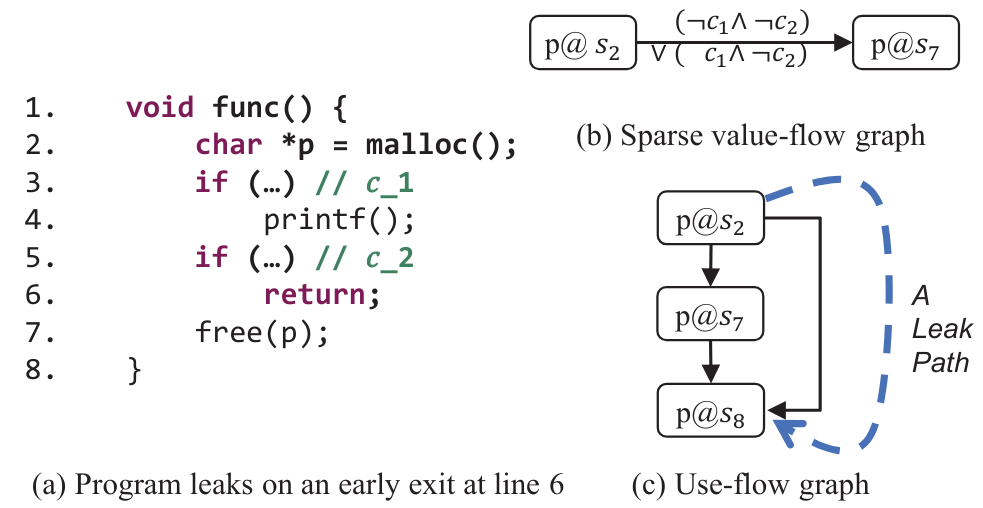
\includegraphics[width=0.6\textwidth]{pic1}
            \caption{Դինամիկ հիշողության արտահոսքի օրինակ}
            \label{fig:figure1}
        \end{figure}

        Երկրորդ փուլում այն օգտագործում է արդեն ստացված UFG֊ի առավել ճշգրիտ վերլուծություն։ Սկզբում որոնում է բոլոր
        ճանապարհները, որոնք չեն պարունակում դինամիկ հիշողություն օգտագործող օպերացիաներ։ Այնուհետև հայտնաբերված յուրաքանչյուր
        ճանապարհի համար կիրառում է Z3 գործիքը\cite{Z3}՝ նրանց իրագործելիությունը ստուգելու համար: Այս գործընթացն անհրաժեշտ է
        ճանապարհների զգայունությունն ապահովելու և կեղծ հայտնաբերված արտահոսքերը զտելու համար։ Գործիքն ունի որոշ սահմանափակումներ՝
        \begin{enumerate}[itemsep=1mm]
            \item Վերլուծությունն արվում է դաշտերի հանդեպ ոչ զգայուն։
            \item Ցուցիչների վերլուծությունը ճշգրիտ չէ։
            \item Որոշ ճանապարհներ անիրագործելի են բարդ թվաբանական և միջֆունկցիոնալ տվյալների կախվածությունների պատճառով։
            \item Հաշվի չի առնվում թվաբանական գործողությունները ցուցիչների հետ, free(p + y) արտահայտությունը համարժեք է համարվում free(p)֊ին, ինչն ակնհայտ սխալ է։
            \item Հաշվի են առվում միայն այն դեպքերը, երբ դինամիկ հիշողության առանձնացման գործողությունը բարեհաջող է անցնում։
        \end{enumerate}

        SMOKE֊ը ծրագրավորված է LLVM-ի վերին մակարդակում և միայն բինար տարբերակն է հասանելի\cite{SMOKE}:

        \subsubsection{PCA}
        CA\cite{Li2020}֊ն առաջին հերթին թարգմանում է նախնական կոդը LLVM IR֊ի։ Այնուհետև, օգտագործելով LLVM֊ի gold plugin֊ը
        բոլոր IR ֆայլերը հավաքում է մեկում։ Ապա այն օգտագործում է Անդերսենի ցուցիչների վերլուծության գործիքը\cite{Andersen}
        և հավաքում ցուցիչների մասին ինֆորմացիա, մասնավորապես, թե որ դինամիկ հիշողության օբյեկտի վրա է հղված այս կամ այն ցուցիչը։
        Այդ ինֆորմացիայի վրա հիմնվելով, կառուցվում են ֆունկցիաների կանչերի կախվածության և ղեկավարման կախվածության գրաֆները։
        Եւ վերջում, արդեն ունենալով համապատասխան գրաֆներն ու ինֆորմացիան, կառուցվում է միջֆունկցիոնալ տվյալների կախվածության գրաֆ(DDG)։

        Դինամիկ հիշողության արտահոսքի հայտնաբերման նպատակով PCA֊ը յուրաքանչյուր դինամիկ հիշողություն առանձնացնող ինստրուկցիայի(A)
        համար հավաքում է բոլոր նրանից հասանելի գագաթները(N) DDG֊ում: Եթե N֊ը առանձնացված հիշողությունն ազատող ինստրուկցիա
        չի ներառում, ապա պնդում է, որ տեղի ունի հիշողության արտահոսք։

        Որոշ դինամիկ հիշողության օբյեկտների կարող են հետևել մեկից ավելի դրանք ազատող ինստրուկցիաներ DDG֊ում։
        Նման դեպքերում, A֊ն կհամարվի ազատված, եթե գոյություն ունի ղեկավարման կախվածության ճանապարհ A֊ից դեպի այն ազատող
        ինստրուկցիան։ Հակառակ դեպքում նույնպես պնդում է, որ տեղի ունի հիշողության արտահոսք։ Գործիքն ունի հետևյալ սահմանափակումները՝
        \begin{enumerate}[itemsep=1mm]
            \item Վերլուծությունն արվում է հոսքի, դաշտի և համատեքստի հանդեպ ոչ զգայուն։
            \item Այն օգտագործում է LLVM gold plugin֊ը IR ֆալերը մեկում հավաքելու համար, այնուհետև կառուցում է DDG, ինչը գործիքը դարձնում է ոչ մասշտաբային։
            Գործիքի նախնական կոդը հասանելի է\cite{PCA}։
        \end{enumerate}

        \subsubsection{SVF}
        SVF\cite{Sui2016}֊ն հիմնված է LLVM֊ի վերին մակարդակում։ Առաջին քայլում այն թարգմանում է նախնական կոդը LLVM IR֊ի։
        Այնուհետև, օգտագործելով LLVM֊ի gold plugin֊ը բոլոր IR ֆայլերը հավաքում է մեկում։ SVF֊ն օգտագործում է որոշ ցուցիչների
        անալիզատորներ, ցուցիչների համար համապատասխան ինֆորմացիա հավաքելու նպատակով, մասնավորապես, թե որ դինամիկ հիշողության
        օբյեկտի վրա է հղված այս կամ այն ցուցիչը։ Անալիզատորներցի մեկն Անդերսենի ցուցիչների անալիզատորն է\cite{Andersen}։
        Օգտագործելով LLVM IR֊ը և ցուցիչների մասին հավաքված ինֆորմացիան՝ գործիքը կառուցում է ղեկավարման կախվածության գրաֆ(CFG)
        և հավաքում է հիշողության ստատիկ առանձին վերագրման մասին ինֆորմացիան(SSA - Static Single Assignment)։
        Յուրաքանչյուր VFG֊ի գագաթ իրենի ներկայացնում է ծրագրի որևէ ինստրուկցիա, իսկ գագաթների միջև կողերը տեղադրվում են
        օգտվելով օգտագործման֊հայտարարման և ցուցիչների մասին հավաքված ինֆորմացիայից։

        Բացի այդ, SVF-ն ապահովում է հիշողության տարածքների տարանջատում, ինչը թույլ է տալիս օգտվողներին հիշողությունը բաժանել
        հավաքածուների: Սա օգտակար է մեծածավալ ծրագրերը վերլուծելու համար, եթե հաշվի է առնվում հիշողության որոշակի տարածք:

        Տարբեր ստուգման գործիքներ կարող են իրականացվել VFG֊ի հիման վրա, որը հասանելի է օգտվող ծրագրերի համար:
        Հիշողության արտահոսքի հայտնաբերումը համարվում է աղբյուր-ստացողի խնդիր (յուրաքանչյուր հիշողության հատկացում
        յուրաքանչյուր ուղու վրա պետք է հասնի իր ազատմանը): Ստորև նշված են գործիքի որոշ սահմանափակումներ՝
        \begin{enumerate}[itemsep=1mm]
            \item Այն օգտագործում է LLVM gold plugin֊ը IR ֆալերը մեկում հավաքելու համար, այնուհետև կառուցում է DDG,
            ինչը գործիքը դարձնում է ոչ մասշտաբային։
            \item Վերլուծությունն արվում է ճանապարհների և դաշտերի հանդեպ ոչ զգայուն։
        \end{enumerate}
    }


    \section{Ծրագրային կոդի հատկությունների հարցումների համակարգի նախագծում}\label{sec:queryEngineDesign}
        {
        Ծրագրային կոդի հատկությունների հարցումների համակարգի նախագծումը բաղկացած է երկու հիմնական փուլերից (Նկար \ref{fig:figure2})`
        \begin{enumerate}
            \item տվյալների հավաքագրում
            \item հարցումների համակարգ
        \end{enumerate}

        \begin{figure}[h]
                \centering
                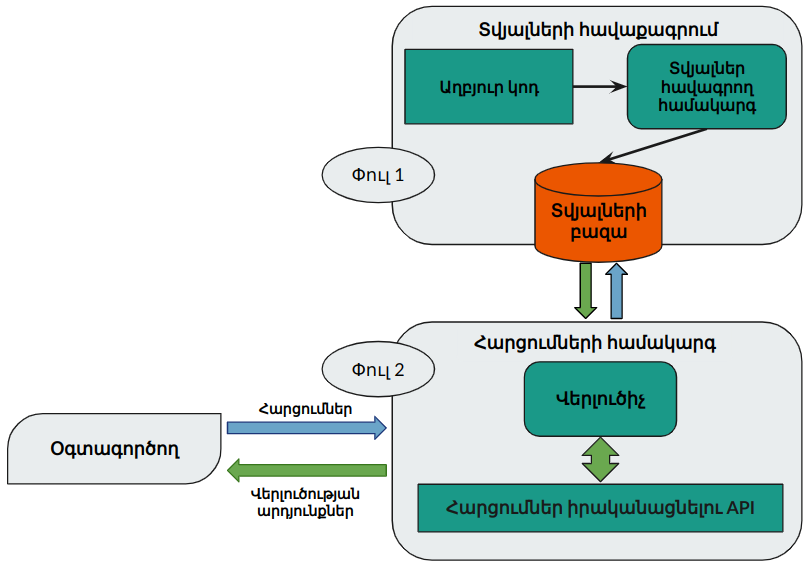
\includegraphics[width=1\textwidth]{pic2}
                \caption{Հարցումների համակարգի նախագծման փուլերը}
                \label{fig:figure2}
        \end{figure}

        Առաջին փուլը տվյալների հավաքագրման փուլն է, որի նպատակն է ստեղծել տվյալների բազա, որը կպահի աղբյուր կոդի
        վերաբերյալ անհրաժեշտ տեղեկությունները:
        Բազմաթիվ բաց կոդով նախագծերից իրականացվում է տվյալների հավաքագրում.
        աղբյուր կոդից ստանալով անհրաժեշտ տեղեկություններ պահպանում ենք դրանք տվյալների բազայում:

        Երկրորդ փուլը բուն hարցումների համակարգի նախագծումն է: Այս փուլում մշակվում է հարցումների համակարգ, որի միջոցով
        օգտագործողները կատարելով հարցումներ կարող են վերլուծել իրենց ծրագրերի հատկությունները:

        {
    \subsection{Տվյալների հավաքագրում}\label{subsec:dataCollection}
    Ծրագրային կոդի հատկությունների հարցումների համակարգի համար էական դեր ունի տվյալների հավաքագրման փուլը
    (Նկար \ref{fig:figure5}): Այս փուլում  կարևոր է տվյալներ հավաքագրող համակարգի
    օգտագործումը: Տվյալներ հավաքագրող համակարգի նպատակն է վերլուծել ծրագրային կոդը և հավաքագրել անհրաժեշտ
    տեղեկություններ՝ ներառյալ ծրագրի կառուցվածքի, ղեկավարման հոսքի և ներքին փոխկապակցվածությունների վերաբերյալ։

    \begin{figure}[h]
        \centering
        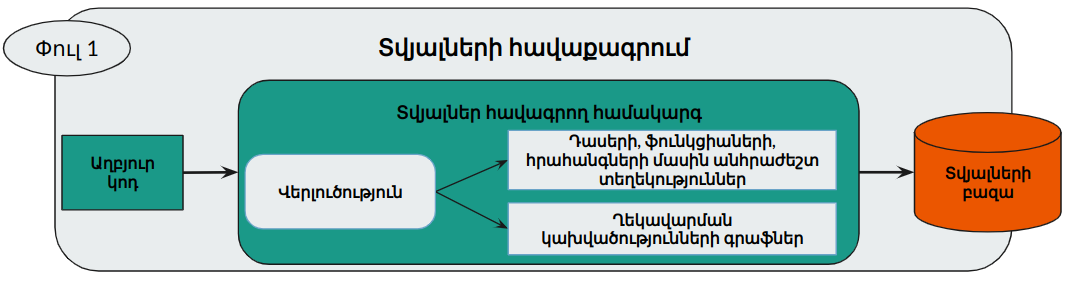
\includegraphics[width=1\textwidth]{pic5}
        \caption{Փուլ 1, տվյալների հավաքագրում}
        \label{fig:figure5}
    \end{figure}

    Տվյալներ հավաքագրող համակարգը մուտքում ստանում է աղբյուր կոդի ֆայլերը և իրականացնում վերլուծություններ՝
    ընդգրկելով հետևյալ տեղեկությունների հավաքագրումը.
    \begin{enumerate}
        \item Դասերի մասին տեղեկություններ՝ ներառյալ յուրաքանչյուր դասի անունը, դասի դաշտերը,
        աղբյուր կոդի տողերի համարները, ժառանգականության կապերը, ֆունկցիաները և այլն,
        \item Ֆունկցիաների մասին տեղեկություններ՝ ներառյալ յուրաքանչյուր ֆունկցիայի անունը, վերասահմանված ֆունկցիա լինելը,
        աղբյուր կոդի տողերի համարները, հայտարարող դասի անունը, կանչվող ֆունկցիաները, արգումենտները, լոկալ փոփոխականները,
        օգտագործվող և սահմանվող դաշտերը, տեսանելիությունը և այլն:
        \item Հրահանգների մասին տեղեկություններ՝ ներառյալ յուրաքանչյուր հրահանգների տիպը, աղբյուր կոդի տողերը,
        կանչվող ֆունկցիաները, օպերանդները, օգտագործվող և սահմանվող փոփոխականները և այլն:
    \end{enumerate}

    Այս տվյալները պահվում են կառուցված տվյալների բազայում՝ հետագա վերլուծությունների և հարցումների համար
    օգտագործելու նպատակով: Դրանք հիմք են հանդիսանում ծրագրային կոդի հատկությունների հարցումների համակարգի համար:

    {
    \subsubsection{Տվյալների բազայի նախագծում}\label{subsubsec:database}

    Հարցումները արդյունավետ կատարելու նպատակով տվյալների բազայի նախագծում՝ հաշվի առնելով ռելացիոն ու ոչ ռելացիոն
    բազաների հատկությունները։

    \begin{figure}[h]
        \centering
        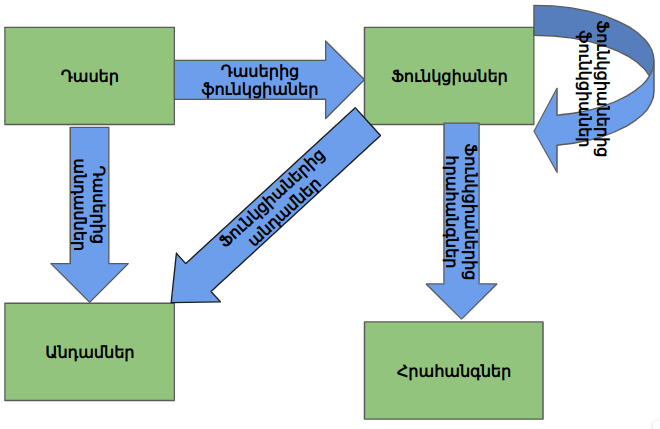
\includegraphics[width=0.8\textwidth]{pic7}
        \caption{Տվյալների բազայի կառուցվածքը}
        \label{fig:figure7}
    \end{figure}
}

%    {

}
}

        {
    \subsubsection{Հարցումների խմբեր}\label{subsubsec:queryGroups}
    {
    \subsubsection{Հարցումների խմբեր}\label{subsubsec:queryGroups}
    Գրել բաժանումների մասին

    \phantomsection
    \subsubsection*{Դասերի համար հարցումներ}\label{subsubsec:classes}
    \addcontentsline{toc}{subsubsection}{Դասերի համար հարցումներ}
    Կլասների հարցումների մասին խոսել։

    \phantomsection
    \subsubsection*{Ֆունկցիաների համար հարցումներ}\label{subsubsec:functions}
    \addcontentsline{toc}{subsubsection}{Ֆունկցիաների համար հարցումներ}
    Ֆունկցիաների հարցումների մասին խոսել։

    \phantomsection
    \subsubsection*{Հրահանգների համար հարցումներ}\label{subsubsec:instructions}
    \addcontentsline{toc}{subsubsection}{Հրահանգների համար հարցումներ}
    Ինստրուկցիաների հարցումների մասին խոսել։

    \phantomsection
    \subsubsection*{Օգտագործողի կողմից կառավարվող տվյալների վերլուծության հարցումներ}\label{subsubsec:taintAnalisys}
    \addcontentsline{toc}{subsubsection}{Օգտագործողի կողմից կառավարվող տվյալների վերլուծության հարցումներ}
    Ավելացնել ալգորիթմերի բարդությունը։
}
}
    }



    \section{Ծրագրային կոդի հատկությունների հարցումների համակարգի իրականացում}\label{sec:queryEngineImplementation}
    {
	\subsubsection{Հարցումների ավտոմատ գեներացման համակարգ}\label{subsubsec:queryAggregation}
	{

}

	\subsubsection{Բսղադրյալ գրաֆ}\label{subsubsec:proceduregraph}
	{
	\subsection{Բաղադրյալ գրաֆ}\label{subsec:proceduregraph}
	Ծրագրային կոդի հատկությունների վերլուծություններն իրականացնելու համար օգտագործվել է բաղադրյալ գրաֆ կառուցվածքը։
	Բաղադրյալ գրաֆն ուղորդված գրաֆ է, որի գագաթները ներկայացնում են միջանկյալ ներկայացման   հրամաններ, ֆունկցիայի պարամետրեր,
	գլոբալ փոփոխականներ, դասի անդամ փոփոխականներ, իսկ կողերը ցույց են տալիս գրաֆի գագաթների միջև ղեկավարման և
	տվյալային կախվածությունները (Նկար \ref{fig:figure8}):

	\begin{figure}[h]
		\centering
		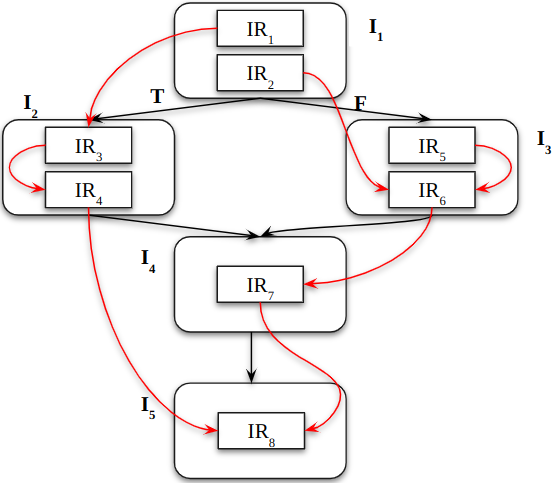
\includegraphics[width=0.7\textwidth]{pic8}
		\caption{Բաղադրյալ գրաֆ}
		\label{fig:figure8}
	\end{figure}

	Բաղադրյալ գրաֆը կառուցվում է ղեկավարման հոսքի գրաֆի հիման վրա, նրան ավելացնելով հավելյալ գագաթներ և կողեր։
	Ավելացվող գագաթներն իրենցից ներկայացնում են այն գլոբալ փոփոխականների կամ դասերի դաշտերի հայտարարումները, որոնից
	գրաֆի գագաթներին համապատախանող հրահանգներում առկա է տվյալային կախվածություն։ Ավելացվող կողերը ցույց են տալիս գրաֆի
	գագաթներին համապատասխանող հրահանգների միջև առկա տվյալային կախվածությունները։

	Ծրագրի հրահանգների փոխարեն, որպես բաղադրյալ գրաֆի գագաթներ են օգտագործվել միջանկյալ ներկայացման հրամանները։
	Այդ կերպ բարձրացվել է կատարվող վերլուծությունների ճշտությունը։  Նկար \ref{fig:figure9}-ում ներկայացված է աղբյուր կոդը
	և այդ կոդի բաղադրյալ գրաֆը։ Ինչպես երևում է բաղադրյալ գրաֆից, ֆունկցիայի կողմից վերադրաձվող v2 փոփոխականի արժեքը
	հաստատուն է և կախված չէ ֆունկցիայի x արգումենտից։

	\begin{figure}[h]
		\centering
		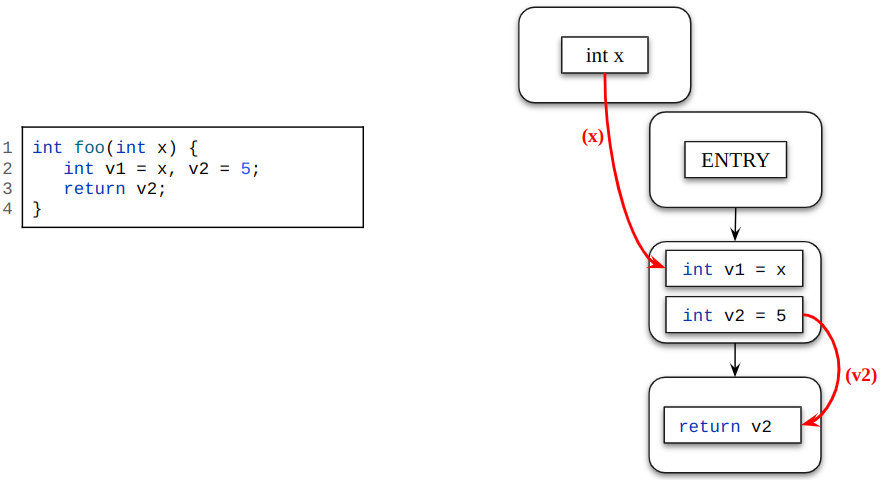
\includegraphics[width=1\textwidth]{pic9}
		\caption{Աղբյուր կոդ օրինակ և համապատասխանող բաղադրյալ գրաֆը}
		\label{fig:figure9}
	\end{figure}

	\subsubsection{Տվյալների հոսքի վերլուծություն}
	
	Տվյալների հոսքի վերլուծությունը ծրագրի կատարման ճանապարհներին տվյալների հոսքերի մասին ինֆորմացիայի հավաքագրումն է։
	Այն կատարվում է ղեկավարման հոսքի գրաֆի հիման վրա։ Տվյալների հոսքի վերլուծության երկու հիմնական մեթոդներն են ակտիվ
	փոփոխակաների և հասնող սահմանումների\cite{aho} վերլուծությունները։ Գործիքում տվյալների հոսքի վերլուծությունը
	կատարվել է  ակտիվ փոփոխականների վերլուծությամբ։
	
	\subsubsection{Ակտիվ փոփոխականների վերլուծություն}
	
	Փոփոխականն ակտիվ է ծրագրի որոշակի կետում, եթե իրեն վերագրված արժեքը ղեկավարման հոսքի գրաֆում իր ժառանգների կողմից օգտագործվում է:
	Վերլուծություն կատարելու համար օգտագործում ենք հետևյալ չորս բազմությունները՝ \textit{def}, \textit{use}, \textit{in} և \textit{out}։
	Ղեկավարման հոսքի V գագաթի def բազմությունը պարունակում է այն փոփոխականները, որոնք արժեքավորվել են V գագաթում,
	իսկ use բազմությունը՝ որոնք օգտագործվել են V գագաթում։ Ունենալով այս երկու բազմությունները, կարող ենք հաշվել in և out
	բազմությունները (այսինքն ակտիվ փոփոխականների բազմությունը գագաթ մուտք գործելիս և գագաթից դուրս գալիս),
	հետևյալ հավասարումների միջոցով\cite{aho}.
	
	{		
		\vspace{-\baselineskip}	
		\begin{align*}
			&\text{IN}[exit] = \varnothing & \\
			&\text{IN}[V] = \text{use}[V] \cup (\text{OUT}[V] \setminus \text{def}[V]) & \\
			&\text{OUT}[V] = \bigcup_{s \in \text{V}{successors}} \text{IN}[s] & 
		\end{align*}
	}

	Նկատենք, որ in և out բազմությունները հաշվելու հավասարումները ռեկուրսիվ են և փոխկապակցված։ Առաջին հավասարումը
	սահմանում է սահմանային պայմանը։ Սա նշանակում է, որ ծրագրի ավարտին ակտիվ փոփոխականներ չկան։ Երկրորդ հավասարումով
	ասվում է, որ փոփոխականը գագաթ մուտք գործելիս ակտիվ է, եթե այն օգտագործվում է գագաթում, կամ դուրս է գալիս գագաթից
	առանց վերասահմանվելու։ Երրորդ հավասարումով ասվում է, որ գագաթից դուրս գալիս փոփոխականն ակտիվ է այն և միայն այն
	դեպքում, երբ այն ակտիվ է իր ժառանգ գագաթներից գոնե մեկում։
	
	\subsubsection{def և use բազմություններ}
	Յուրաքանչյուր գագաթում առկա փոփոխականները դիտարկվում են կամ  որպես սահմանվող(def) կամ որպես օգտագործվող(use)
	փոփոխականներ։ Որոշ  փոփոխականներ դիտարկվում են և որպես սահմանվող, և որպես օգտագործվող փոփոխակներ։ Օրինակ, եթե
	դիտարկենք “++” post increment օպերատորը, “var++” արտահայտությունում var փոփոխականը և օգտագործվում է և նորից
	սահամանվում։ Դիտարկված փոփոխականներն ավելացվում են def և use բազմություններում։

	Այսպիսով կատարվում է def և use փոփոխականների վերլուծություն և ղեկավարման հոսքի գրաֆի յուրաքանչյուր գագաթի համար
	տրվում է այդ գագաթի def և use բազմությունները։ Նկար \ref{fig:figure10}-ում ցուցադրված է Նկար \ref{fig:figure9}-ի
	օրինակին համապատասխանող def և use բազմությունները։

	\begin{figure}[h]
		\centering
		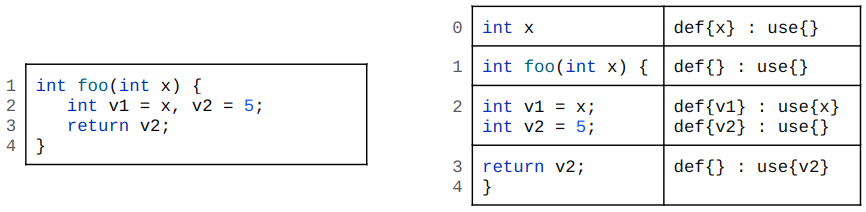
\includegraphics[width=1\textwidth]{pic10}
		\caption{def և use բազմություններ}
		\label{fig:figure10}
	\end{figure}
	
}
}



    \section{Վիճակի փոփոխության վրա հիմնված սխալների հայտնաբերում}\label{sec:bugDetection}
    {
    \subsection{Թեստավորում}\label{subsec:testing}
    {
    \subsection{Թեստավորում}\label{subsec:testing}
    Մշակված գործիքը թեստավորվել և համեմատվել է աշխարհում արդեն գոյություն ունեցող այլ գործիքների հետ։ Ինչպես նաև գործիքի
    միջոցով թեստավորվել են բաց կոդով հասանելի ավելի քան 100 պրոեկտ, որոնք իրականացված են մեծամասամբ C ծրագրավորման լեզվով։

    \subsubsection{Արդյունքների համեմատումը Juliet թեստերի հավաքածույի վրա}
    MLH֊ը թեստավորվել է Juliet թեստերի հավաքածույի վրա, որը նախատեսված է ծրագրային ապահովման գործիքների թեստավորման և
    արդյունքների գնահատման համար։ Այն Software Assurance Metrics and Tool Evaluation(SAMATE)\cite{SAMATE} նախագծի մասն է
    կազմում, որը մշակվել է National Institue of Standards and Technology(NIST)֊ի կողմից։ Ջուլիետ թեստերի հավաքածուն
    ներառում է ավելի քան 120,000 թեստերի օրինակներ առանձնացված զանազան խնդիրների համար ինչպիսիք են դինամիկ հիշողության
    արտահոսքը, բուֆերի գերհագեցումը և այլն։ Այն ներառում է թեստեր C/C++, Java և Ada լեզուներով:
    Թեստավորման համար հավաքածուից առանձնացվել են միայն դինամիկ հիշողության արտահոսքի համար նախատեսված
    օրինակները (CWE401\_Memory\_Leak\cite{CWE401}): Մշակվել է թեստավորման համակարգ, որը գնահատում է ունեցած գործիքների
    արդյունավետությունը վերը նշված հավաքածուի համար։ Ստորև ներկայացված է առաջատար այլ գործիքների և
    նոր մշակված գործիքի արդյունավետության աղյուսակը (Աղյուսակ\ref{tab:juliet_test}):
    \begin{table}[h!]
    \centering
    \begin{tabularx}{\textwidth}{|*{6}{>{\centering\arraybackslash}X|}}
        \hline
        \textbf{Name} & \textbf{True Positives} & \textbf{True Negatives} & \textbf{False Positives} & \textbf{False Negatives} & \textbf{F1 score} \\
        \hline
        \textbf{CSA} & 536 & 4481 & 125 & 332 & 0.7011 \\
        \hline
        \textbf{Infer} & 262 & 4392 & 214 & 606 & 0.3899 \\
        \hline
        \textbf{SMOKE} & 496 & 4510 & 96 & 372 & 0.6795 \\
        \hline
        \textbf{PCA} & 486 & 4342 & 264 & 382 & 0.6007 \\
        \hline
        \textbf{SVF} & 452 & 4168 & 438 & 416 & 0.5142 \\
        \hline
        \rowcolor{yellow!100} \textbf{MLH} & 868 & 4606 & 0 & 0 & 1 \\
        \hline
    \end{tabularx}
    \caption{Juliet թեստերի հավաքածույի վրա համեմատման արդյունքների}
    \label{tab:juliet_test}
\end{table}
}

    \subsection{Արդյունքներ}\label{subsec:results}
    {
    \subsection{Արդյունքներ}\label{subsec:results}
    Ստորև ներկայացված է առաջատար այլ գործիքների և
    նոր մշակված գործիքի արդյունավետության աղյուսակը (Աղյուսակ\ref{tab:juliet_test}):
    \begin{table}[h!]
    \centering
    \begin{tabularx}{\textwidth}{|*{6}{>{\centering\arraybackslash}X|}}
        \hline
        \textbf{Name} & \textbf{True Positives} & \textbf{True Negatives} & \textbf{False Positives} & \textbf{False Negatives} & \textbf{F1 score} \\
        \hline
        \textbf{CSA} & 536 & 4481 & 125 & 332 & 0.7011 \\
        \hline
        \textbf{Infer} & 262 & 4392 & 214 & 606 & 0.3899 \\
        \hline
        \textbf{SMOKE} & 496 & 4510 & 96 & 372 & 0.6795 \\
        \hline
        \textbf{PCA} & 486 & 4342 & 264 & 382 & 0.6007 \\
        \hline
        \textbf{SVF} & 452 & 4168 & 438 & 416 & 0.5142 \\
        \hline
        \rowcolor{yellow!100} \textbf{MLH} & 868 & 4606 & 0 & 0 & 1 \\
        \hline
    \end{tabularx}
    \caption{Juliet թեստերի հավաքածույի վրա համեմատման արդյունքների}
    \label{tab:juliet_test}
\end{table}

    \subsubsection{Դինամիկ հիշողության արտահոսքի հայտնաբերումը առաջատար բաց կոդով գործիքներում}
    Մի շարք հատուկ առանձնացված բաց կոդով գործիքներ դասակարգված են ըստ իրենց ակտիվության և կարևորության։ Այդ գործիքներից
    ավելի քան հարյուրը թեստավորվել են նոր մշակված գործիքի միջոցով՝ դինամիկ հիշողության արտահոսքի խնդիրները հայտնաբերելու
    նպատակով։ Ստացված արդյունքները հավելյալ ստուգվել են աշխատակիցների կողմից։ Ստացված ճիշտ արդյունքները հրապարակվել և
    հաստատվել են, սխալ ստացված արդյունքների համար կատարվել է վերլուծություն և մշակվել հետագա պլան գործիքում առկա
    թերությունները վերացնելու նպատակով։ Նկար \ref{fig:figure4}-ում ներկայացված է ֆունկցիայի օրինակ
    coturn\cite{COTURN}-ից, որում հարցումների համակարգի API-ի օգտագործմամբ գրված
    սստուգիչի կողմից հայտնաբերվել է դինամիկ հիշողության արտահոսքի դեպք։

    \begin{figure}[h]
        \centering
        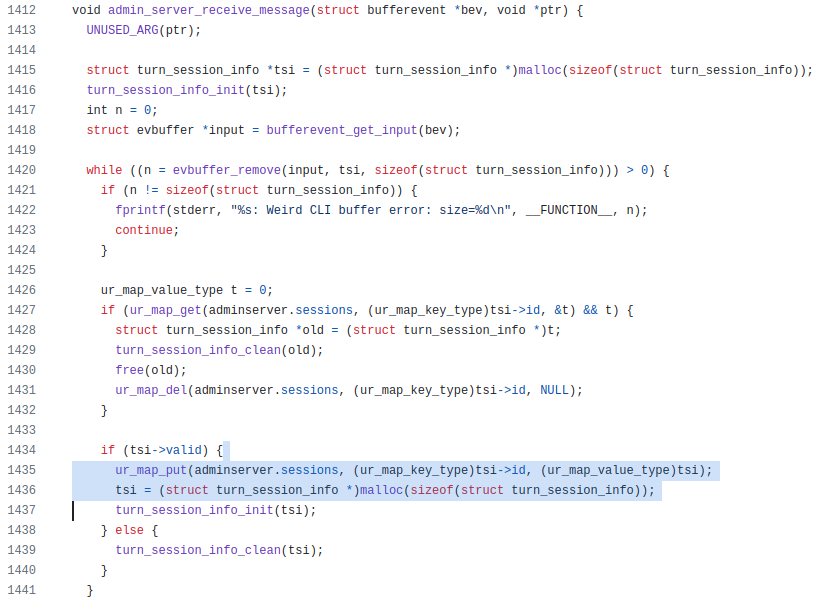
\includegraphics[width=1\textwidth]{pic4}
        \caption{Դինամիկ հիշողության արտահոսքի իրական օրինակ}
        \label{fig:figure4}
    \end{figure}
}
}


    \section{Արդյունքներ}\label{sec:results}
    {
    \subsection{Թեստավորում}\label{subsec:testing}
    {
    \subsection{Թեստավորում}\label{subsec:testing}
    Մշակված գործիքը թեստավորվել և համեմատվել է աշխարհում արդեն գոյություն ունեցող այլ գործիքների հետ։ Ինչպես նաև գործիքի
    միջոցով թեստավորվել են բաց կոդով հասանելի ավելի քան 100 պրոեկտ, որոնք իրականացված են մեծամասամբ C ծրագրավորման լեզվով։

    \subsubsection{Արդյունքների համեմատումը Juliet թեստերի հավաքածույի վրա}
    MLH֊ը թեստավորվել է Juliet թեստերի հավաքածույի վրա, որը նախատեսված է ծրագրային ապահովման գործիքների թեստավորման և
    արդյունքների գնահատման համար։ Այն Software Assurance Metrics and Tool Evaluation(SAMATE)\cite{SAMATE} նախագծի մասն է
    կազմում, որը մշակվել է National Institue of Standards and Technology(NIST)֊ի կողմից։ Ջուլիետ թեստերի հավաքածուն
    ներառում է ավելի քան 120,000 թեստերի օրինակներ առանձնացված զանազան խնդիրների համար ինչպիսիք են դինամիկ հիշողության
    արտահոսքը, բուֆերի գերհագեցումը և այլն։ Այն ներառում է թեստեր C/C++, Java և Ada լեզուներով:
    Թեստավորման համար հավաքածուից առանձնացվել են միայն դինամիկ հիշողության արտահոսքի համար նախատեսված
    օրինակները (CWE401\_Memory\_Leak\cite{CWE401}): Մշակվել է թեստավորման համակարգ, որը գնահատում է ունեցած գործիքների
    արդյունավետությունը վերը նշված հավաքածուի համար։ Ստորև ներկայացված է առաջատար այլ գործիքների և
    նոր մշակված գործիքի արդյունավետության աղյուսակը (Աղյուսակ\ref{tab:juliet_test}):
    \begin{table}[h!]
    \centering
    \begin{tabularx}{\textwidth}{|*{6}{>{\centering\arraybackslash}X|}}
        \hline
        \textbf{Name} & \textbf{True Positives} & \textbf{True Negatives} & \textbf{False Positives} & \textbf{False Negatives} & \textbf{F1 score} \\
        \hline
        \textbf{CSA} & 536 & 4481 & 125 & 332 & 0.7011 \\
        \hline
        \textbf{Infer} & 262 & 4392 & 214 & 606 & 0.3899 \\
        \hline
        \textbf{SMOKE} & 496 & 4510 & 96 & 372 & 0.6795 \\
        \hline
        \textbf{PCA} & 486 & 4342 & 264 & 382 & 0.6007 \\
        \hline
        \textbf{SVF} & 452 & 4168 & 438 & 416 & 0.5142 \\
        \hline
        \rowcolor{yellow!100} \textbf{MLH} & 868 & 4606 & 0 & 0 & 1 \\
        \hline
    \end{tabularx}
    \caption{Juliet թեստերի հավաքածույի վրա համեմատման արդյունքների}
    \label{tab:juliet_test}
\end{table}
}
}


    \section{Հետագա աշխատանք}\label{sec:furtherWork}
    {
	\clearpage
	\section{Հետագա աշխատանք}\label{sec:furtherWork}
	Նախատեսվում է \ldots \\
	\\
	Այժմ աշխատանք է տարվում \ldots
}

    \clearpage
    \phantomsection
    \section*{Եզրակացություն}\label{sec:conclusion}
    \addcontentsline{toc}{section}{Եզրակացություն}
    {
	\begin{enumerate}
		\item
		Նախագծվել և իրականացվել է ծրագրային կոդի հատկությունների հարցումների համակարգ,

		\item
		Օգտագործելով հարցումների համակարգը` ստեղծվել է դինամիկ հիշողության արտահոսքի սխալների հայտնաբերման ալգորիթմ

        {
			\begin{enumerate}
				\item
				Թեստավորվել են C լեզվով գրված` բաց կոդով հասանելի 100 նախագծերի վրա (top 100 by github stars), որի արդյունքում հայտնաբերվել են սխալներ։
			\end{enumerate}
		}

	\end{enumerate}
}


    \clearpage
    \phantomsection
    \addcontentsline{toc}{section}{Գրականություն}
    \bibliographystyle{plainnat}
    \bibliography{bibliography}
\end{document}